\section{Evaluación tiempo de lectura de datos usando APIs}
El tipo de prueba que se realizó es el mismo que el utilizado por \cite{tesis-cerda-rodrigo}, por tanto se considera como ciclo de lectura cuando el software de control Arduino, envía los valores de todos los flexores agregados, esto es realizado en paralelo a la lectura de todos los datos que entrega el IMU. Cada medición considera el tiempo transcurrido desde la generación del mensaje en el software de control hasta que llega a la API de alto nivel. Se realizaron 1000 pruebas de ciclos lectura utilizando un Baudrate de 57600, un LoopDelay igual a 0 ms y Threshold igual a 0 en la placa Arduino. Se realizaron pruebas con el IMU enviando la información completa (acelerómetro, giroscopio y magnetómetro) y modificando la cantidad de flexores desde uno a 1 a 10, siendo simulados con solo un sólo flexor físico en la placa. El dispositivo utilizado para la evaluación técnica de las APIs fue el Samsung Galaxy S5 Mini.

\subsection{API C\#}
%Flexores e IMU update resources

% {START} RESUME TABLE ---------------------------------
%\caption[Resumen resultado pruebas de lectura flexores e IMU usando API C\# ]{Resumen resultado pruebas de lectura flexores e IMU usando API C\#  en $\mu s$\\ Fuente: Elaboración propia (2018)}
%\label{table:flexors&imu-xamarin-galaxy-api}

% Table created by stargazer v.5.2.2 by Marek Hlavac, Harvard University. E-mail: hlavac at fas.harvard.edu
% Date and time: Tue, Sep 04, 2018 - 17:29:17
\begin{table}[!htbp] \centering 
\caption[Resumen resultados de pruebas de lectura flexores e IMU usando API C\#]{Resumen resultados de pruebas de lectura flexores e IMU usando API C\# en $\mu s$\\ Fuente: Elaboración propia (2018)}
\label{table:flexors&imu-xamarin-galaxy-api}
\begin{tabular}{@{\extracolsep{5pt}} cccccccc} 
\\[-1.8ex]\hline 
\hline \\[-1.8ex] 
flexors & Mean & Median & Min & Max & Std. Dev. & Skewness & Kurtosis \\ 
\hline \\[-1.8ex] 
$1$ & $16,038.830$ & $15,068.100$ & $7,417.900$ & $28,865.600$ & $4,484.658$ & $0.692$ & $2.908$ \\ 
$2$ & $1,365.986$ & $1,271.700$ & $376.800$ & $3,635.400$ & $704.429$ & $0.816$ & $3.307$ \\ 
$3$ & $3,133.853$ & $2,734.500$ & $895.200$ & $8,272.900$ & $1,636.889$ & $1.166$ & $3.906$ \\ 
$4$ & $5,251.955$ & $4,796.100$ & $1,605$ & $12,720.200$ & $2,327.944$ & $0.877$ & $3.417$ \\ 
$5$ & $7,391.620$ & $6,823.100$ & $2,496.400$ & $16,335.200$ & $2,972.165$ & $0.739$ & $3.123$ \\ 
$6$ & $9,445.057$ & $8,723.800$ & $3,565$ & $20,047.800$ & $3,703.347$ & $0.815$ & $3.074$ \\ 
$7$ & $11,231.080$ & $10,768.700$ & $4,948.100$ & $21,445.900$ & $3,611.584$ & $0.609$ & $2.891$ \\ 
$8$ & $12,864.060$ & $12,476.600$ & $6,264.900$ & $24,091.800$ & $3,660.714$ & $0.646$ & $3.045$ \\ 
$9$ & $14,512.320$ & $14,120.300$ & $7,632.200$ & $27,282$ & $4,010.673$ & $0.657$ & $2.891$ \\ 
$10$ & $15,967.690$ & $15,187.800$ & $9,808$ & $27,444.800$ & $3,769.420$ & $0.806$ & $3.086$ \\ 
\hline \\[-1.8ex] 
\end{tabular} 
\end{table} 
% {END} RESUME TABLE ---------------------------------

La Figura \ref{fig:xamarin-galaxy-hist-flexor&imu-api}, muestra los histogramas de las latencias obtenidas al recibir los mensajes de los flexores e IMU, modificando la cantidad de flexores de uno a diez.

\begin{figure}
 \begin{center} 
   	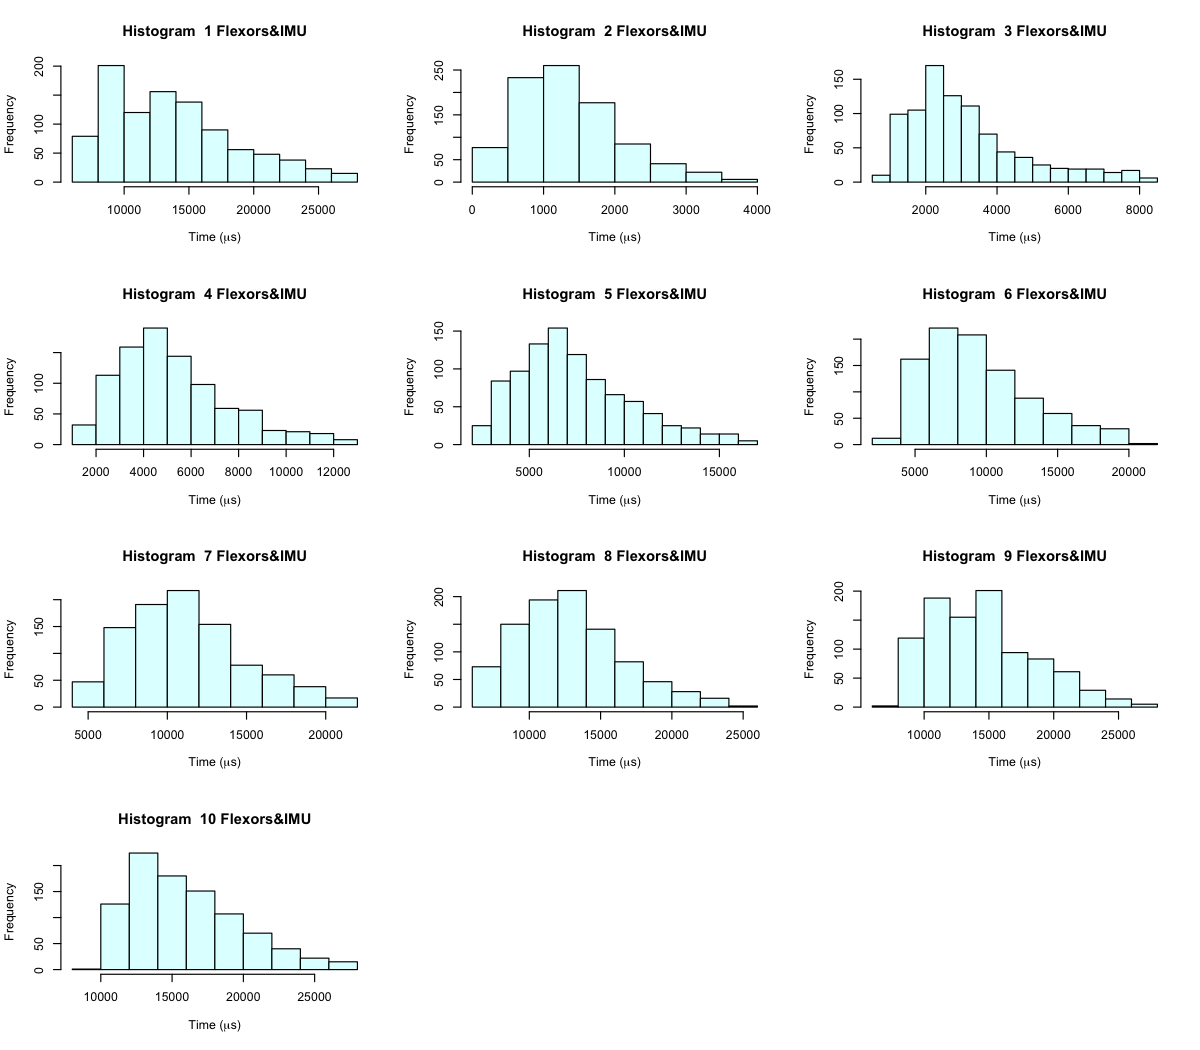
\includegraphics[width=1.0\textwidth]{evaluation/graphics/Xamarin/Galaxy-APITest/HistFlexors&IMUXamarinGalaxy-APITest.png}
   \centering
    \caption[Histogramas de Flexores e IMU usando API C\#]{Histogramas de Flexores e IMU usando API C\# \\Fuente: elaboración propia (2018)}
    \label{fig:xamarin-galaxy-hist-flexors&imu-api}
  \end{center}
\end{figure}

\begin{figure}[H]
  \begin{center} 
   	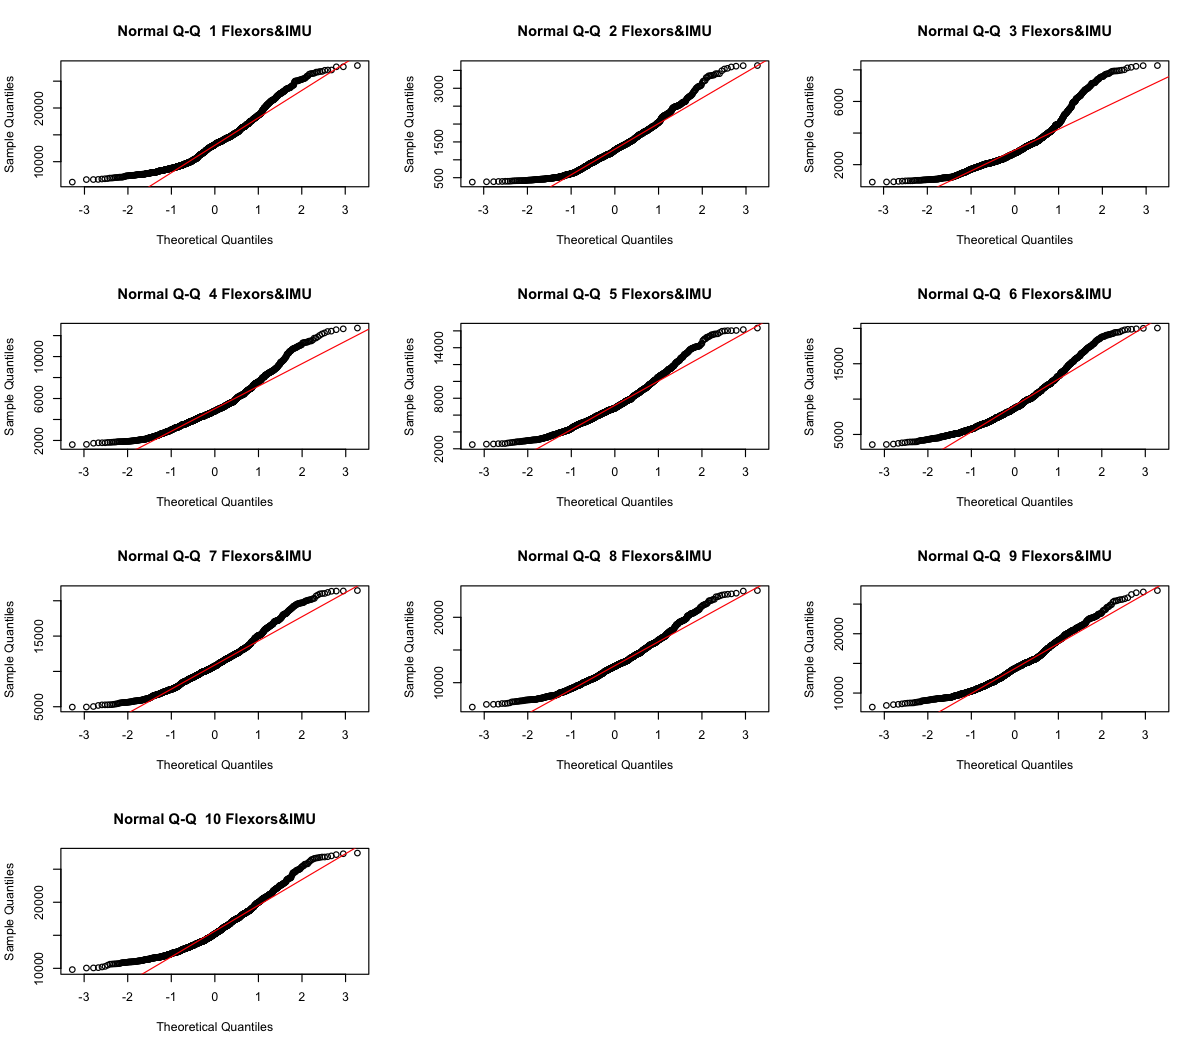
\includegraphics[width=1.0\textwidth]{evaluation/graphics/Xamarin/Galaxy-APITest/NormalQQFlexors&IMUXamarinGalaxy-APITest.png} 
   	\centering
    \caption[Gráfico QQ de Flexores e IMU usando API C\# ]{Flexores e IMU usando API C\# \\Fuente: elaboración propia (2018)} 
    \label{fig:xamarin-galaxy-QQ-flexors&imu-api}
  \end{center}
\end{figure}

\begin{figure}[H]
  \begin{center} 
   	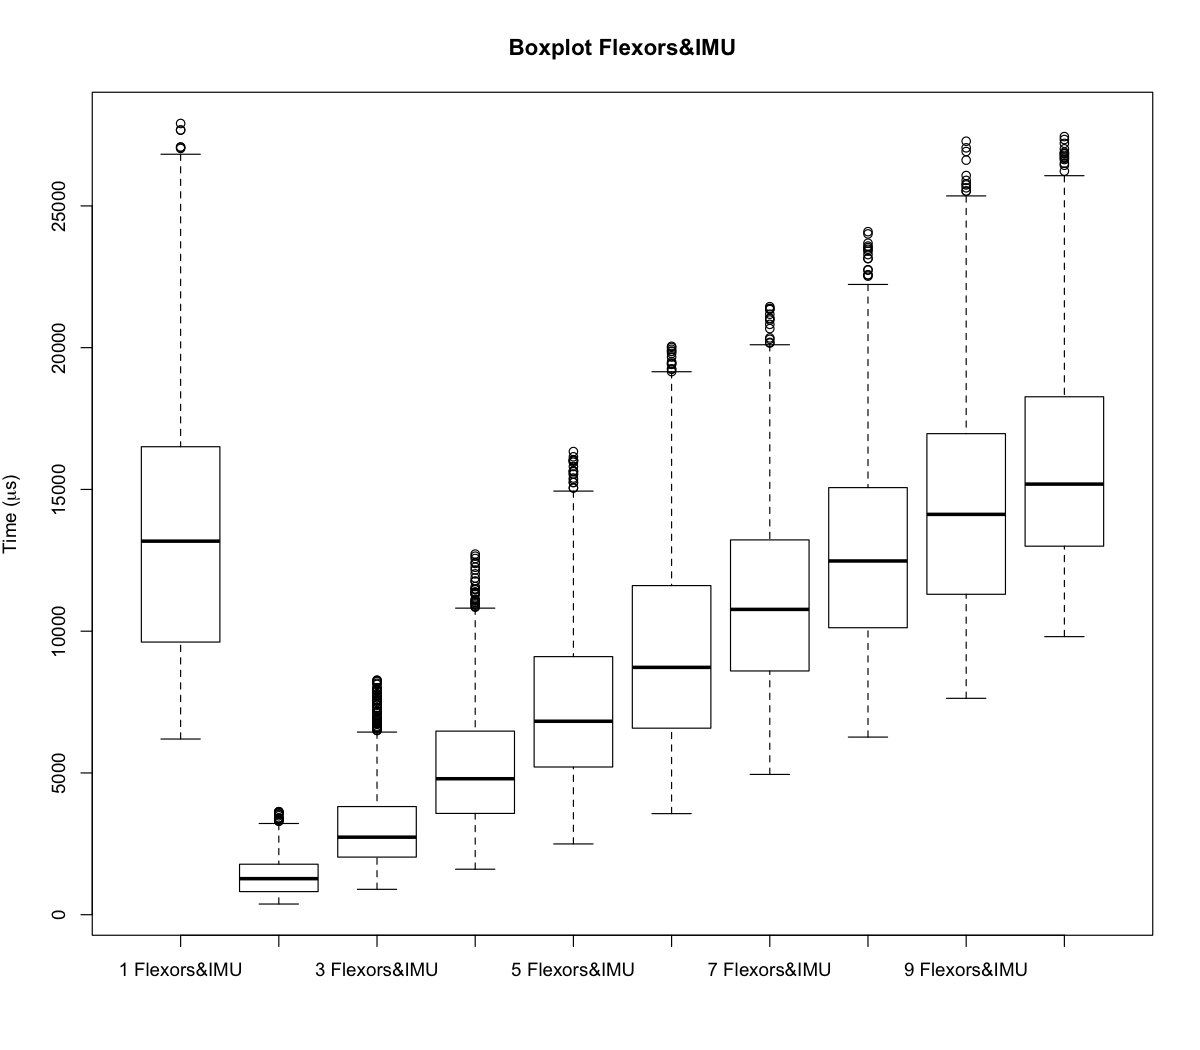
\includegraphics[width=0.8\textwidth]{evaluation/graphics/Xamarin/Galaxy-APITest/BoxplotFlexors&IMUXamarinGalaxy-APITest.png} 
   	\centering
    \caption[Gráficos de cajas de Flexores e IMU usando API C\#  ]{Gráficos de cajas de Flexores e IMU usando API C\# \\Fuente: elaboración propia (2018)} 
    \label{fig:xamarin-galaxy-boxplot-flexors&imu-api}
  \end{center}
\end{figure}

\subsection{API Java}